\subsection{Cam-Clay consolidation with swelling}
As before, equations \ref{eq:H2liq} and \ref{eq:H2gas} define the fluid system. In this example, however, we choose a numerical solution in OpenGeoSys that accomodates pressure variables in the solution vector. Both equations are therefore algebraically manipulated so that the primary variables to solve for are now the capillary pressure, $p_c$, and the non-wetting pressure, $p_{nw}$,

\begin{equation}
\phi {{\rho }_{w}}\frac{\partial {{S}_{w}}}{\partial {{p}_{c}}}\frac{d{{p}_{c}}}{dt}+{{\rho }_{w}}{{S}_{w}}\nabla \cdot \frac{d\mathbf{u}}{dt}+\nabla \cdot \left[ {{\rho }_{w}}\frac{\mathbf{k}k_{w}^{r}}{{{\mu }_{w}}}\left( -\nabla {{p}_{nw}}+\nabla {{p}_{c}}+{{\rho }_{w}}\mathbf{g} \right) \right]={{Q}_{w}}
\end{equation}

\begin{equation}
\begin{split}
%\begin{align}
  & -\phi {{\rho }_{nw}}\frac{\partial {{S}_{w}}}{\partial {{p}_{c}}}\frac{d{{p}_{c}}}{dt}+\phi \left( 1-{{S}_{w}} \right)\left( \frac{\partial {{\rho }_{nw}}}{\partial {{p}_{nw}}}\frac{d{{p}_{nw}}}{dt}+\frac{\partial {{\rho }_{nw}}}{\partial {{p}_{c}}}\frac{d{{p}_{c}}}{dt} \right)+ \\ 
 & \text{          }\left( {{\rho }_{w}}{{S}_{w}}+{{\rho }_{nw}}\left( 1-{{S}_{w}} \right) \right)\nabla \cdot \frac{d\mathbf{u}}{dt}+\nabla \cdot \left[ {{\rho }_{nw}}\frac{\mathbf{k}k_{nw}^{r}}{{{\mu }_{nw}}}\left( -\nabla {{p}_{nw}}+{{\rho }_{nw}}\mathbf{g} \right) \right]={{Q}_{nw}} \\ 
%\end{align}
\end{split}
\end{equation}

where in this case we assume that solid grains are incompressible. 

As in Section 14.2, swelling stress is based on the linear swelling model proposed by Rutqvist (2005) \cite{Jonny05}, which defines the increment of swelling stress to be proportional to liquid saturation increment,

\begin{equation}
\Delta \sigma ^{sw}=\beta \Delta S_w,
\end{equation}

where $\beta $ is a swelling coefficient that could be called the maximum swelling stress. As the saturation change approaches unity, swelling stress approaches $\beta $.

\subsubsection*{Definition}
Fig. \ref{fig_aximodel} shows the axi-symmetric model domain for the confined swelling test as well as the initial and boundary conditions for the two-phase flow consolidation problem with hydraulic and fluid properties are given in Table \ref{tab:hydromat}. The parameters of the elasto-plastic swelling model are given in Table \ref{tab:pls} for Cam-Clay plasticity.

\begin{figure}[!tbh]
\centering
\scalebox{0.5} % Change this value to rescale the drawing.
{
\begin{pspicture}(0,-8)(17.45797,8)
\psframe[linewidth=0.04,dimen=outer](10,7.5)(7,-7.5)
\usefont{T1}{ptm}{m}{n}
\rput(8.526719,0.1696875){
\begin{minipage}{0.12\textwidth}
{\color{blue}
\begin{align*}
&p^c=84.6\mbox{MPa}\\
&p^g=0.1\mbox{MPa}
\end{align*}
}
{\color{red}
\begin{align*}
&\sigma_x=0.1\mbox{MPa}\\
&\sigma_y=0.1\mbox{MPa}\\
&\sigma_z=0.1\mbox{MPa}\\
&\sigma_{xy}=0\\
&\sigma_{yz}=0\\
&\sigma_{zx}=0
\end{align*}
}
\end{minipage}
}
\usefont{T1}{ptm}{m}{n}
\rput{90.0}(6.5,-6)
{\rput(6.5,0.6696875){{\color{blue}${\partial p^c}/{\partial x}=0,\, {\partial p^g}/{\partial x}=0$},{\color{red}$\,u_x=0,\, \sigma_{xy}=0$}}}
\usefont{T1}{ptm}{m}{n}
\rput{90.0}(12,-11.5)
{\rput(12,0.6696875){{\color{blue}${\partial p^c}/{\partial x}=0,\, {\partial p^g}/{\partial x}=0$},{\color{red}$\,u_x=0,\, \sigma_{xy}=0$}}}
\usefont{T1}{ptm}{m}{n}
\rput(8.757343,8){{\color{blue}${\partial p^c}/{\partial y}=0,\, p^g=0.1\mbox{MPa}$},{\color{red}$\,u_y=0,\, \sigma_{xy}=0$}}
\usefont{T1}{ptm}{m}{n}
\rput(8.757343,-8){{\color{blue}$p^c=0,\, p^g=0.1\mbox{MPa}$},{\color{red}$\,u_y=0,\, \sigma_{xy}=0$}}
\end{pspicture}
}
\caption{Model set-up with initial and boundary conditions.}
\label{fig_aximodel}
\end{figure}

\begin{table}[!htb]
\centering
\begin{tabular}{lll}
\hline\noalign{\smallskip}
Meaning & Value & Unit \\
\hline
Liquid density, $\rho _{w}$ & $1000$ & $kg/m^3$\\
Liquid viscosity, $\mu_w$ &$10^{-3}$ & $Pa\,s$\\
Gas density,  $\rho _{nw}$ & Clapeyron equation & $kg/m^3$\\
Gas viscosity, , $\mu _{nw}$ &$1.8\times10^{-5}$ & $Pa\,s$\\
Intrinsic permeability, $k$ & $0.6\times10^{-20}$ & $m^2$\\
Porosity, $\phi $ & $0.4$ & $m^3/m^3$ \\
Media properties for liquid: &  & \\
\textit{Relative permeability} & Power law $k_{w}^r=S_e^3$  & \\
Residual saturation & 0 &--- \\
Maximum saturation & 1 &--- \\
\textit{Water retention} & van Genuchten  & \\
Exponential index, $m$ & 0.42 &--- \\
Air entry pressure, $p_0$& 62 &$MPa$ \\
Relative permeability of gas, $k_{nw}^r$ & $5.103\times10^{-12}\left[e(1-S^l)\right]^{4.3}$ & $e$, void ratio\\
\hline
\end{tabular}
\caption{Hydraulic properties} %\footnotesize
\label{tab:hydromat}
\end{table}

\begin{table}[!htb]
\centering
\begin{tabular}{lrl}
\hline\noalign{\smallskip}
Parameter & Value & Unit \\
\hline
Slope of the critical state line, $M$ & $1.5$ & ---\\
Virgin compression index, $\lambda_p$ & $1.5$ & ---\\
Swelling/recompression index, $\kappa$ & $0.1$ & ---\\
Initial preconsolidation pressure, $p_c$& $8.0$ & $MPa$\\
Initial void ratio, $e$ & $0.7$ & $--$\\
Poisson ratio & $0.4$ & ---\\
Initial ($s=0$) elastic slope for $1+e-p$, $\kappa_{i0}$& $0.01$ & ---\\
Initial ($\sigma=0$) elastic slope for $1+e-s$, $\kappa_{s0}$& $0.25$ & ---\\
Minimum bulk modulus, $K_{min}$ & $10$ &$MPa$\\
First parameter for $\kappa_s$, $\alpha_{ss}$ & $-0.03$ & $MPa^{-1}$\\
Second parameter for $\kappa_s$, $\alpha_{sp}$ & $-0.1609$ & ---\\
Parameter for $\kappa_i$, $\alpha_{i}$ & $-0.003$ & $MPa^{-1}$\\
Reference mean stress, $p_{ref}$ & $0.1$ & $MPa$\\
\hline
\end{tabular}
\caption{Plasticity parameters for the Cam-Clay model} %\footnotesize
\label{tab:pls}
\end{table}

\subsubsection*{Results}
Fig. \ref{fig:S_top} shows the temporal evolution of water saturation on the bottom of the sample between OpenGeoSys and Code-Bright.

\begin{figure}[!thb]
\begin{center}
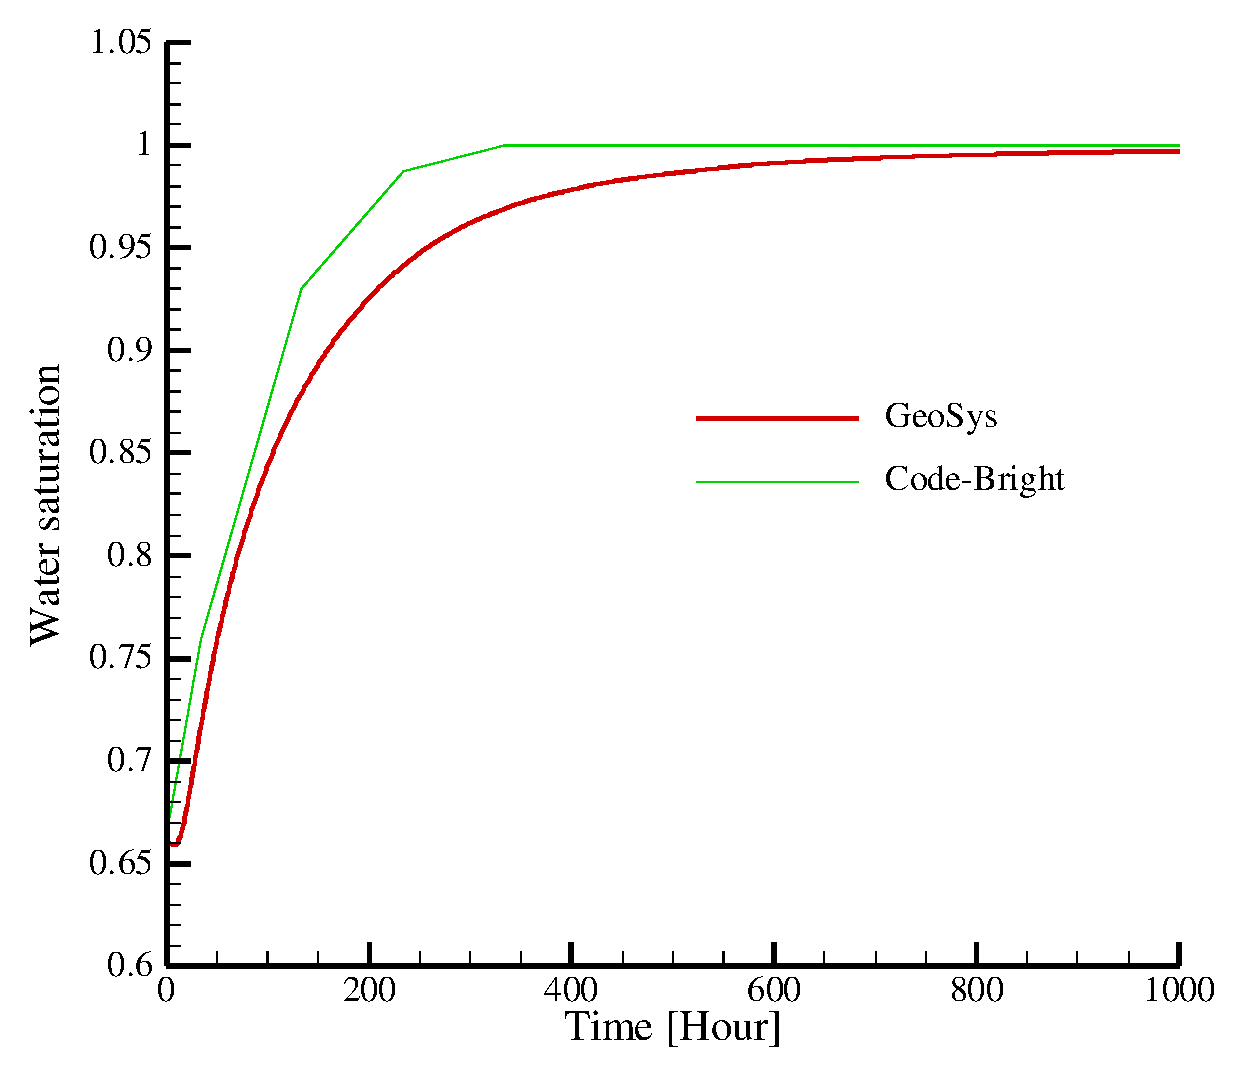
\includegraphics[width=0.7\textwidth]{chapter_14/figures/fig_14_3_25}
\end{center}
\caption{Water saturation evolution at the sample bottom.}
\label{fig:S_top}
\end{figure}